\section{Introdução + Porque consideramos interessante}

O trabalho aqui apresentado desenvolve o pensamento de uma aplicação de um manipulador industrial Stäubli TX90, em uma linha de produção robótica construída para a pintura de bandeiras do Brasil. Este trabalho foi desenvolvido considerando muitos fatores da atualidade, tais como as condições de trabalho humanas atuais em grandes linhas de produção, a busca pela qualidade e consistência de produtos, a automatização de processos e aumento de vendas de produtos sazonais para a Copa do Mundo FIFA 2026.

Como visto ao longo da matéria de Robótica Industrial, ministrada pela professora Ludmila Corrêa de Alkmin e Silva, robôs industriais têm tomado cada vez mais a linha de frente de grandes linhas produtivas, principalmente em processos repetitivos, de alta velocidade e que exigem um nível de padrão no tempo (INTERNATIONAL FEDERATION OF ROBOTICS, 2026). Substituindo manufaturas que antes dependiam totalmente de trabalho humano e braçal. Isso ocorre devido ao grande número de inconsistências que uma produção humana em processos repetitivos pode trazer, especialmente quando há fadiga, esforço físico contínuo e necessidade de manter ritmo constante de produção. Essa tensão entre trabalho humano, repetição e velocidade industrial é satirizada por Charlie Chaplin em Tempos Modernos, filme em que o operário tenta acompanhar o ritmo de uma linha de montagem mecanizada (CHAPLIN, 1936). 

Apesar de não estarmos tratando aqui de uma atividade simples como apertar um parafuso (a qual um robô muito mais simples poderia realizar), a pintura de um padrão em uma sequência de movimentos idêntica durante um longo período de tempo traz uma fadiga natural da mente e resiliência humana e com esta diversas alterações na qualidade do produto. Isto não considera ainda o ambiente de trabalho, que muitas vezes apresenta riscos para aquelas pessoas que estão na frente do produto, realizando a pintura de fato. Risco este que pode ser, neste caso, químico, pela grande quantidade de inaláveis que estão presentes nas tintas utilizadas para pintura, físico, pelas longas horas tendo de realizar movimentos repetitivos, e mental, uma vez que a maioria destes trabalhadores tem que realizar suas funções em locais que não são os mais bem preparados para realizarem pausas, pela natureza do produto utilizado ou ainda que estimulem de alguma maneira o desenvolvimento daquele trabalhador em quesitos intelectuais.

Uma diferença fundamental do tempo de Chaplin para os dias de hoje, é o fato de que atualmente temos robôs que não apenas podem aparafusar um parafuso, mas também realizar movimentos que a pouco tempo atrás seriam considerados irreais. Enquanto temos robôs que são projetados para substituir simples ações, que muitas vezes podem ser realizadas por até um robô de 3 graus de liberdade, temos outros com seis ou mais eixos, capazes de realizar atividades de complexidade muito maior, quando aplicável. Assim, a automação da pintura indústrial não se justifica apenas pelo aumento da produtividade alcançada pelos manipuladores, que são limitados apenas em sua configuração, mas também pela melhoria das condições de trabalho e pela redução da variação entre produtos.

Em outro espectro de análise, temos a questão da alteração sazonal do mercado consumidor causado por alguns eventos importantes. A cada 4 anos, o mundo assiste ao maior espetáculo esportivo de todos, a Copa do Mundo FIFA. Um evento que não apenas altera o mercado brasileiro, como o mundial. E nesta sazonalidade, o mercado tem que se adaptar para vender milhões de produtos temáticos ligados à identidade visual e nacional de cada país. Entre os mais comprados no Brasil, está a bandeira do Brasil, item muito comemorado como maior representatividade possível ao país pelo qual o torcedor está dando seu apoio. 

Isto é comprovado por pesquisas de consumo que indicam aumento na intenção de compra de produtos ligados à Copa do Mundo, como camisas da Seleção Brasileira, bandeiras, acessórios e itens temáticos, especialmente no período próximo aos jogos (RODRIGUES; FRITOLI, 2022; CNDL; SPC BRASIL; OFFERWISE, 2026). Esta demanda concentrada em um período limitado exige que a indústria consiga aumentar a produção mantendo a qualidade e repetibilidade de seus produtos que não tem esta demanda tão constante ao longo do ano. Para isto, é necessário então implementar uma automação robótica deste processo, melhorando a cadência produtiva e ao mesmo tempo não expondo pessoas desnecessariamente às condições já discutidas anteriormente.

Juntando estas duas perspectivas, a de automatizações de linha de trabalho e substituição de tarefas realizadas anteriormente por pessoas, agora por robôs especializados, e a de necessidade de aumento da produção de produtos, em especial da bandeira do Brasil para a Copa do Mundo, o grupo decidiu por tomar como projeto a implementação de um robô industrial para realizar a pintura de bandeiras do Brasil em uma linha de produção, para que a demanda do mercado seja atendida e uma eficiência maior seja alcançada. Dessa forma, a escolha da bandeira do Brasil como padrão de pintura torna a aplicação interessante não só pelo tema, mas também porque traz uma situação real de aumento de produção em uma linha industrial.

Falando do ponto de vista técnico também, a bandeira parece uma boa escolha pois reúne diferentes tipos de trajetórias em uma mesma tarefa. As definições de limites da bandeira podem ser representadas por formas geométricas não muito complexas, como o retângulo, losango, círculo e faixa curva. Este conjunto de geometrias exige uma realização completa de movimentos do manipulador, como segmentos retilíneos, mudanças de direção, contornos fechados e trajetórias curvas. além disso, como a pintura envolve mais de uma cor, tendo que trocar do verde para o amarelo, para o azul e branco, a operação completa também exige deslocamentos suaves, diferente dos deslocamentos aproximadamente constantes sendo utilizados na pintura, até a estação de troca de ferramenta ou pistola. Mostrando assim um leque completo de realização de atividades diferentes pelo manipulador.

Para o desenvolvimento do projeto, de uma maneira a equivaler os padrões de qualidade da indústria, a lógica de movimentação considerada é composta por velocidade aproximadamente constante durante a aplicação da tinta na bandeira e trajetórias suaves durante os deslocamentos entre o local de pintura e a troca de ferramentas ou cores. Esta distinção de lógicas de movimentações é importante para essa aplicação, uma vez que a pintura exige uma variação mínima de velocidade ao longo da deposição da tinta, por conta de diferenças que a velocidade pode ocasionar na qualidade uniforme da pintura desejada. Já nos movimentos sem aplicação de tinta, o objetivo muda, sendo agora a prioridade deslocar o efetuador de maneira segura e eficiente até o ponto de troca, evitando movimentos desnecessários ou bruscos, por precaução de danificar os equipamentos de pistola de tinta na troca ou chegada para pintura.

Uma vez definido o tema e atividade a ser realizada pelo grupo, foi necessário encontrar um robô industrial que pudesse ser implementado em uma linha de produção para realizar esta tarefa. Os principais parâmetros considerados foram: possuir 6 graus de liberdade, ter um posicionamento do efetuador e uma orientação da ferramenta de aplicação em um mesmo robô, ter um alcance de aproximadamente 1 metro, boa repetibilidade e carga suficiente para carregar o aplicador de tinta e seus suportes. Na simulação foi adotada uma ferramenta de $3{,}0\,\text{kg}$, mantendo margem em relação à carga nominal do robô, para um cenário onde uma ferramenta de maior carga possa ser utilizada.

Após realizar a busca pelo modelo ideal, a equipe acabou por decidir utilizar o modelo Staübli TX90. Este modelo apresenta todos os pontos desejados pela equipe. Ele tem 3 de seus graus de liberdade voltados para realizar o posicionamento do atuador no espaço e 3 graus de liberdade reservados para realizar a orientação da ferramenta utilizada, (o que é perfeito para a aplicação desejada, pois o robô não deve apenas chegar nos pontos desejados da bandeira, como também deve ser capaz de manter a posição e orientação corretos em relação à superfície sendo pintada ao longo da trajetória) área de atuação de $1000\,\text{mm}$, repetibilidade de aproximadamente $\pm0{,}03\,\text{mm}$ e carga nominal de $7\,\text{kg}$ \cite{staubli2017}. A carga também é um ponto importante, uma vez que o braço deve carregar a pistola de pintura, o suporte e os demais elementos instalados na flange. Uma margem também é importante aqui para possíveis outras aplicações.

Este modelo acaba por ser o fit perfeito, não apenas pelos pontos citados, mas também por apresentar em sua ficha técnica a aplicação de pintura … . Além disso, a divisão dos graus de liberdade na maneira já falada permite a aplicação de pintura de formatos necessários para a bandeira do Brasil, como o losango, o quadrado e o círculo. Não apenas isto, mas como o braço também terá de realizar troca de pistolas, para trocar de cor ao longo do processo. Pedindo assim um sistema de que seja capaz de acompanhar traçados, realizar mudanças de direção, contornos fechados e trajetórias curvas, seguindo caminhos pré-determinados e também alterando sua velocidade de aproximadamente  constante para suave, quando necessário. Tarefas as quais o Staübli TX90 é totalmente capaz de realizar, com os controles, comandos e programas corretos.

Alguns outros robôs também foram analisados para esta tarefa, com os dois principais concorrentes sendo o FANUC P-40iA e o Yaskawa Motoman MPX1150. O FANUC P-40iA é um robô de pintura de seis eixos, com carga de até $5\,\text{kg}$ e alcance aproximado de $1300\,\text{mm}$. O Yaskawa Motoman MPX1150, por sua vez, é um robô compacto de seis eixos voltado à pintura, com carga de até $5\,\text{kg}$ e alcance horizontal de $727\,\text{mm}$ \cite{fanuc2026,yaskawa2026}.

Estas diferenças podem ser mais bem visualizadas na tabela a seguir:


\begin{table}[H]
\centering
\small
\caption{Comparação entre robôs analisados para a tarefa}
\begin{tabularx}{\textwidth}{|p{2.2cm}|p{3.1cm}|p{1.3cm}|p{1.7cm}|X|X|}
\hline
 \textbf{Robô} & \textbf{Tipo de aplicação} & \textbf{Carga útil} & \textbf{Alcance aproximado} & \textbf{Pontos fortes para a tarefa} & \textbf{Limitações em relação ao projeto} \\ \hline
 Staubli TX90 & Manipulador industrial articulado de uso geral, com aplicacao prevista em pintura & 7 kg & 1000 mm & Boa repetibilidade, 6 GDL, porte compativel com celula de pecas pequenas/medias, maior margem de carga para ferramenta e suportes, referencias de cinemática e simulacao ja disponiveis & Menos especializado em pintura que modelos dedicados; exige maior cuidado na integracao da ferramenta \\ \hline
 FANUC P-40iA & Robo dedicado a pintura em celulas compactas e linhas com variacao de produtos & 5 kg & 1300 mm & Especializado em pintura, adequado a pequenos lotes, mudancas de estilo e espacos reduzidos & Menor margem de carga que o TX90; menor disponibilidade de referencias cinematicas ja estudadas pelo grupo \\ \hline
 Yaskawa Motoman MPX1150 & Robo compacto dedicado a pintura de componentes menores e contornados & 5 kg & 727 mm & Especializado em acabamento consistente e pintura de pecas menores & Alcance menor; pode exigir posicionamento mais restrito da peca ou da celula \\ \hline
\end{tabularx}
\end{table}



Apesar de ambos modelos de comparação aqui serem bons candidatos a realizarem a ação do TX90, ele apresenta capacidades muito equilibradas e mais que suficientes para nosso caso de uso. Ele não irá necessariamente realizar pintura de grandes superfícies com geometrias extremamente complexas, como é o esperado da aplicação dos competidores, mas sim irá trabalhar com padrões mais simples. Além disso, enquanto os outros são muito mais especializados para atuarem com pintura, o manipulador escolhido brilha também na sua versatilidade. 

Na nossa análise, de aumento de produtividade para o evento sazonal não pode depender apenas de uma etapa na linha produtiva, mas sim contar com a automação de mais etapas, como o recorte, o preenchimento da pintura (uma vez que para fins de projeto, estamos apenas pintando as delimitações da bandeira aqui), o empacotamento, a dobra, para aumentar a produtividade geral, o que demandaria um pedido maior de máquinas ao fabricante, barateando o custo de compra dos manipuladores. Sendo assim, escolher um robô que é mais versátil e menos especializado em uma única atividade, pode ser um fator importante dentro do problema que buscamos resolver.

Ademais, como se trata de um produto de alta sazonalidade, o fator da configurabilidade dos manipuladores robóticos é bem importante aqui, uma vez que ao final desta sazonalidade a linha de produção montada pode ser re-utilizada, para pintar outros tipos de bandeira (economizando altamente comparado ao custo de moldes de impressão), montagem de peças, acabamentos, entre outras aplicações, desde que estejam dentro da área máxima de atuação dele e abaixo dos 318 Nm de torque máximo das juntas.

Também é possível comparar o TX90 com outros tipos de robôs, como cartesianos ou SCARA. Porém, apesar de ambos terem suas aplicações em que podem entregar o papel desejado com alta eficiência, para nossa tarefa eles não contam com um controle de orientação de pistola desejado para uma tarefa de precisão como a pintura. Como nosso objetivo envolve trajetórias suaves, retas, inclinadas e curvas, além de ter que realizar a troca da cor na pistola, um manipulador de 6 graus de liberdade se mostra a melhor opção.

\section{Revisão bibliográfica}

\subsection{Manipuladores Robóticos Industriais}

Para podermos chegar a conclusão do melhor manipulador para nossa aplicação, necessitamos entender o que é um robô industrial. De maneira geral, um robô industrial pode ser definido como um manipulador automaticamente controlado, reprogramável e multipropósito, programável em 3 ou mais eixos e pode ser fixo ou móvel e utilizado em aplicações de automação industrial \cite{ifr2026}. Esta definição é importante, uma vez que evidencia que o robô industrial não é apenas uma máquina que realiza um único trabalho, mas sim um equipamento que pode ser programado e reprogramado para diferentes funções e operações dentro de uma mesma linha de produção.

Manipuladores robóticos são compostos por elos conectados por juntas. Essas juntas podem ser ou rotativas, ou prismáticas. As rotativas produzem um movimento angular, enquanto as prismáticas produzem um movimento linear. No caso dos manipuladores seriais, elos e juntas formam uma cadeia aberta, o que significa que o movimento de cada junta influenciará diretamente na posição e orientação do efetuador final. Enquanto nos de cadeia fechada o movimento de uma junta pode restringir o movimento das demais. Assim, manipuladores de cadeia aberta acabam sendo muito utilizados para aplicações industriais, por permitirem que ferramentas sejam posicionadas em diferentes regiões no espaço de trabalho e não haja muito movimento desperdiçado.

O número de graus de liberdade de um manipulador está diretamente relacionado com o número de movimentos independentes que ele pode executar. Em um manipulador articulado de seis graus de liberdade, normalmente as 3 primeiras juntas são responsáveis por definir a posição do efetuador, enquanto as últimas 3, a sua orientação. Isto é importante para a aplicação da pintura, além de muitas outras funções, uma vez que isto permite não apenas alcançar um ponto específico, mas também manter uma orientação desejada em relação à superfície de trabalho, neste caso, que está sendo pintada.


\subsection{O manipulador Stäubli TX90}

O manipulador Stäubli TX90 é um manipulador industrial serial articulado composto por seis juntas rotacionais. Sua estrutura permite controlar a pose do efetuador final no espaço, combinando posicionamento e orientação. Pela documentação técnica desta série de manipuladores, podemos ver que ele possui alcance aproximado de 1m (1000mm), carga nominal de 7kg e repetibilidade de aproximadamente $\pm0{,}03\,\text{mm}$ \cite{staubli2017}. Essas características explicam por que ele pode ser aplicado em tarefas industriais que exigem repetição de trajetórias, controle de ferramenta e boa precisão.

No estudo realizado por Rodrigues (2019), foi desenvolvido um modelo cinemático deste manipulador com base no desenvolvimento de equações e convenções de Denavit-Hartenberg, validando este com a comparação direta com uma simulação em software RodoDK e com testes em um robô físico também. O trabalho desenvolvido mostrou que os resultados teóricos coincidem com os resultados encontrados em simulação. Porém os testes divergiram do testado no robô real, com uma diferença média de 2,785mm. Apesar de ser uma diferença que foi considerada relevante no trabalho realizado, uma vez que está bem divergente da repetibilidade do robô, deve ser levado em consideração também as condições de teste, a quais apresentaram algumas inconsistências ao longo dos testes e também que fato que o robô não apresentava ficha de manutenção recente. Pontos de atenção necessários para qualquer validação física de manipuladores \cite{rodrigues2019}.

Um outro ponto de importância levantado por Rodrigues é que o TX90 apresenta particularidades geométricas que precisam ser consideradas no modelo cinemático. Diferenças estão sempre presentes quando se simula um manipulador real e não ideal. Isto reforça ainda a importância de representar corretamente a geometria do manipulador, uma vez que qualquer divergência do cálculo de funcionamento e real atuação do robô tem que ser verificada antes de implementar em produção, passando por todas as etapas de validação e funcionamento necessário, para se obter a saída desejada e com erros mínimos.

\subsection{Cinemática direta, cinemática inversa e parâmetros de Denavit-Hartenberg}

Dentro da análise de manipuladores, a cinemática se posiciona como uma das bases de desenvolvimento fundamentais para que a tarefa possa ser realizada pelo manipulador. Ela descreve o movimento do robô sem considerar diretamente as forças e torques responsáveis necessárias para produzir este movimento, permitindo relacionar os valores das juntas com a posição e a orientação final do efetuador. A cinemática direta determina onde o efetuador estará a partir dos valores das juntas, enquanto a cinemática inversa faz o caminho contrário, calculando quais valores de junta são necessários para atingir uma pose desejada. 

Para modelar manipuladores seriais, a convenção de Denavit-Hartenberg é amplamente utilizada, porque permite descrever a geometria do robô por meio de quatro parâmetros associados a cada elo e junta: comprimento do elo, torção do elo, deslocamento e ângulo de junta. Utilizando este quatro parâmetros, construímos então matrizes de transformação homogênea que representam a relação entre os sistemas de coordenadas consecutivos. A multiplicação dessas matrizes fornece então a transformação total entre a base do robô e o efetuador final. 

Em manipuladores de seis graus de liberdade como o TX90, a cinemática inversa é resolvida por desacoplamento cinemático. Essa abordagem separa o problema em duas etapas: primeiro, é calculada a posição do centro do pulso, relacionada às 3 primeiras juntas, em seguida, é calculada a orientação do efetuador, associada às 3 últimas juntas. Essa solução foi mantida como referência teórica. Já na simulação, as poses da trajetória foram resolvidas numericamente, usando a solução anterior como estimativa inicial, o que facilita manter a continuidade entre os pontos \cite{craig2005,siciliano2010}.

No caso desenvolvido neste projeto, da pintura da bandeira do Brasil, a cinemática inversa é particularmente útil. Uma vez que cada ponto do retângulo, losango, círculo ou faixa corresponde a uma posição desejada da ferramenta, associada também a uma orientação adequada. Assim, o robô deve transformar as geometrias planejadas no espaço cartesiano em valores de junta, mantendo o controle da pose do efetuador ao longo da execução de seus movimentos de pintura.


\subsection{Simulação do TX90 e validação de trajetórias}

A simulação do robô escolhido é uma das etapas mais importantes após a definição matemática do planejamento do movimento e do desenvolvimento matemático necessário para realizar a transformação do movimento do robô. Nesta etapa, avaliará se houve alguma falha nas etapas anteriores de definição, testando o movimento, trajetória, velocidade e esforço total, sem que seja necessário testar com um robô real. Isso se torna mais importante ainda uma vez que estamos considerando um manipulador robótico de tamanho relativo e com força para causar ferimentos graves a alguém que possa estar em sua linha de movimento. Assim, nesta etapa será verificado se qualquer erro foi realizado, poupando algum acidente. No caso específico do Stäubli TX90, Hage, Bidaud e Jardin (2012) apresentaram uma simulação do manipulador em ambiente MatLab/Simulink utilizando do SimMechanics, com o objetivo de prever a posição e a trajetória final com alta confiabilidade \cite{hage2012}.

No caso do estudo de Hage, Bidaud e Jardin (2012), foi realizado um esforço em cima de um foco diferente do aqui proposto, foi analisado o fresamento em vez da pintura, porém o estudo serviu como base inicial para que fosse possível ter uma ideia de onde começar os desenvolvimentos de simulação em ambiente virtual. Este ambiente permite observar posições, velocidades, acelerações e torques.

Ademais, o artigo traz a geração de trajetórias no espaço das juntas utilizando da lei da velocidade trapezoidal. Essa abordagem busca produzir movimentos com velocidade controlada e acelerações coerentes, evitando transições bruscas, o que é muito desejável em uma aplicação de pintura, uma vez que mudanças bruscas de velocidade ou aceleração podem afetar a uniformidade e qualidade da camada de tinta aplicada.

Logo, o uso do MATLAB com Robotics System Toolbox é coerente com a linha geral do projeto desenvolvido, pois permite importar o modelo URDF, resolver a cinemática inversa, calcular a dinâmica e animar o movimento. Dessa forma, esse ambiente foi utilizado para simular o TX90, executar as trajetórias da bandeira e coletar dados de movimentação para validação.

\subsection{Pintura robotizada e planejamento de trajetória}

A aplicação da pintura robotizada é uma composta por diversos fatores para ter sua qualidade mantida, e um dos principais impactadores é o planejamento de trajetória. Diferente de uma aplicação mais simples, como se posicionamento ou de pick and place, a pintura exige que o efetuador percorra uma superfície mantendo certos parâmetros dentro da faixa desejada. Alguns desses parâmetros são: a distância entre a ferramenta e a peça, a orientação da pistola em relação à superfície, a velocidade de deslocamento do efetuador, a vazão de tinta e a sobreposição entre passadas.

Chen, Fuhlbrigge e Li (2009) trazem que o planejamento de trajetórias para pintura robotizada influencia na uniformidade de aplicação da camada de tinta, no tempo de ciclo e no desperdício de material. Mais tradicionalmente, muitas trajetórias eram ensinadas manualmente ao robô, processo que pode ser demorado, dependendo da habilidade do operador. Por isso, métodos automáticos baseados em CAD e informações geométricas da peça se tornam importantes para aplicações industriais. Já em superfícies complexas, temos uma dificuldade maior, uma vez que temos que considerar variações de curvatura e limites de peças mais complexos\cite{chen2009}.

Chen e Xi (2008) falam sobre o planejamento automático de trajetórias de ferramentas para pinturas destas superfícies complexas, em seus estudos. Eles levam em consideração o modelo da pistola, a geometria da superfície e os requisitos de espessura da camada a ser aplicada. Estes fatores deixam bem evidente que a pintura deve ser tratada como um problema de geração de trajetória com restrições de processo, e não só como uma movimentação entre pontos, em sistemas potencialmente mais complexos \cite{chenxi2008}.

Outros estudos sobre cobertura uniforme também reforçam que a trejatória da ferramenta deve considerar o padrão de deposição da tinta, o espaço entre passadas e o perfil de velocidade. Atkar et al. (2005) e Conner et al. (2005) falam sobre problemas relacionados à cobertura de superfícies automotivas, nas quais a uniformidade da camada depende da interação a geometria da superfície, o padrão de spary, velocidade e sobreposição \cite{atkar2005,conner2005}.

Esses estudos são importantes para consolidar a visão sobre a aplicação. No entanto, para o trabalho aqui desenvolvido, foi adotada uma aproximação mais simples: a simulação valida o movimento necessário para traçar os contornos, mas não calcula deposição, vazão, sobreposição ou espessura da camada de tinta, para intuito de melhor estudo do funcionamento do manipulador.

\subsection{Exemplos reais e temos inovadores relacionados}

Exemplos muito próximos ao objetivo do nosso trabalho podem ser observados em aplicações nas quais a pintura robotizada não se limita a cobrir uma superfície inteira, mas que precisa aplicar padrões, regiões, ou marcações com repetibilidade. Um bom exemplo disso é a Dürr, que desenvolveu um sistema chamado EcoPaintJet Pro, instalado em um manipulador, para aplicar tinta diretamente sobre áreas escolhidas da carroceria, permitindo pintura em duas cores diferentes, faixas e elementos gráficos também sem o uso tradicional de mascaramento, com uma aplicação muito precisa e sem desperdício de tinta \cite{durr2026}. De maneira parecida, temos o RoadPrintz, que utiliza um robô Yaskawa, com o objetivo de pintar marcações viárias, como símbolos, setas e faixas. Isto mostra a validação da replicabilidade de precisão fornecida por esta implementação, a diferença é que este manipulador está acoplado em um caminhão, para trabalho externo.

Os principais temas inovadores que são abordados na nossa aplicação são a replicação de padrões geométricos com alta fidelidade e confiabilidade, mesmo que estes demandem desafios de movimentação diferentes em uma mesma tarefa geral. Ademais, tratamos em uma mesma aplicação, perfis de velocidade diferentes necessários para a troca da tinta e a atividade de pintura, uma contínua, uma suave, uma vez que etapas diferentes do projeto demandam perfis de atuação diferentes. Isto coloca a nossa aplicação em um patamar não apenas de uma simples simulação de robô desenhando cegamente uma bandeira, mas sim uma implementação de conceitos de robótica que pode vir a ser implementada em uma linha de produção automatizada. Assim o produto final deve conseguir executar trajetórias planejadas, manter controle de pose, diferenciar movimentos de pintura e movimentos de transição e permitir a repetição do padrão com qualidade suficiente para uma linha produtiva de alta demanda.


\section{Métodos}

\subsection{Descrição do robô escolhido}

O manipulador considerado no projeto é o Stäubli TX90, modelado como um robô serial articulado de seis juntas rotacionais. O robô será tratado a partir da sua função específica na linha de produção maior: posicionar e orientar a ferramenta responsável por aplicar tinta sobre a peça, seguindo trajetórias previamente definidas para formar a bandeira do Brasil. Na simulação, o aplicador foi representado por uma carga de $3{,}0\,\text{kg}$ e por um TCP localizado a $0{,}15\,\text{m}$ do flange. A trajetória da ferramenta é definida no espaço cartesiano, enquanto o movimento real do manipulador ocorre por meio da variação angular de suas juntas. Assim, cada ponto da trajetória da bandeira é convertido em uma configuração articular correspondente, por meio do uso da cinemática direta, inversa, do cálculo de velocidades e dinâmica, de modo que o robô seja capaz de posicionar a ferramenta no local correto.

Aqui, a peça a ser pintada foi representada em um sistema X correspondente a direção frente-trás, um eixo Y correspondente as laterais e por fim o eixo Z para o sentido vertical. A geometria da bandeira é composta por um retângulo de 500mm por 700mm, um losango na horizontal dentro da bandeira, um círculo central de raio 122,5mm e uma faixa curva no centro, completando assim a bandeira do Brasil. 

Durante a pintura, a ferramenta se desloca com velocidade limitada a $0{,}12\,\text{m/s}$ e aceleração limitada a $0{,}30\,\text{m/s}^2$. Nos deslocamentos entre a estação e a bandeira, foram adotados os limites de $0{,}35\,\text{m/s}$ e $0{,}60\,\text{m/s}^2$. Na pintura da bandeira, foi utilizada velocidade aproximadamente constante nos trechos centrais, com transições suaves pelo perfil LSPB, para evitar transições muito bruscas e trancos dos atuadores. Já nas transições, foi utilizdo inteiramente o perfil LSPB suave, considerando a necessicade de não ter impacto forte da ferramenta de aplicação.

Estas considerações e escolhas foram feitas para assim podermos representar mais fielmente uma aplicação industrial na dada situação apresentada. Claro, seguindo algumas simplificações dentro do esperado para o projeto, mas mantendo ainda os principais passos que uma aplicação dessas demandaria.
\begin{figure}[H]
    \centering
    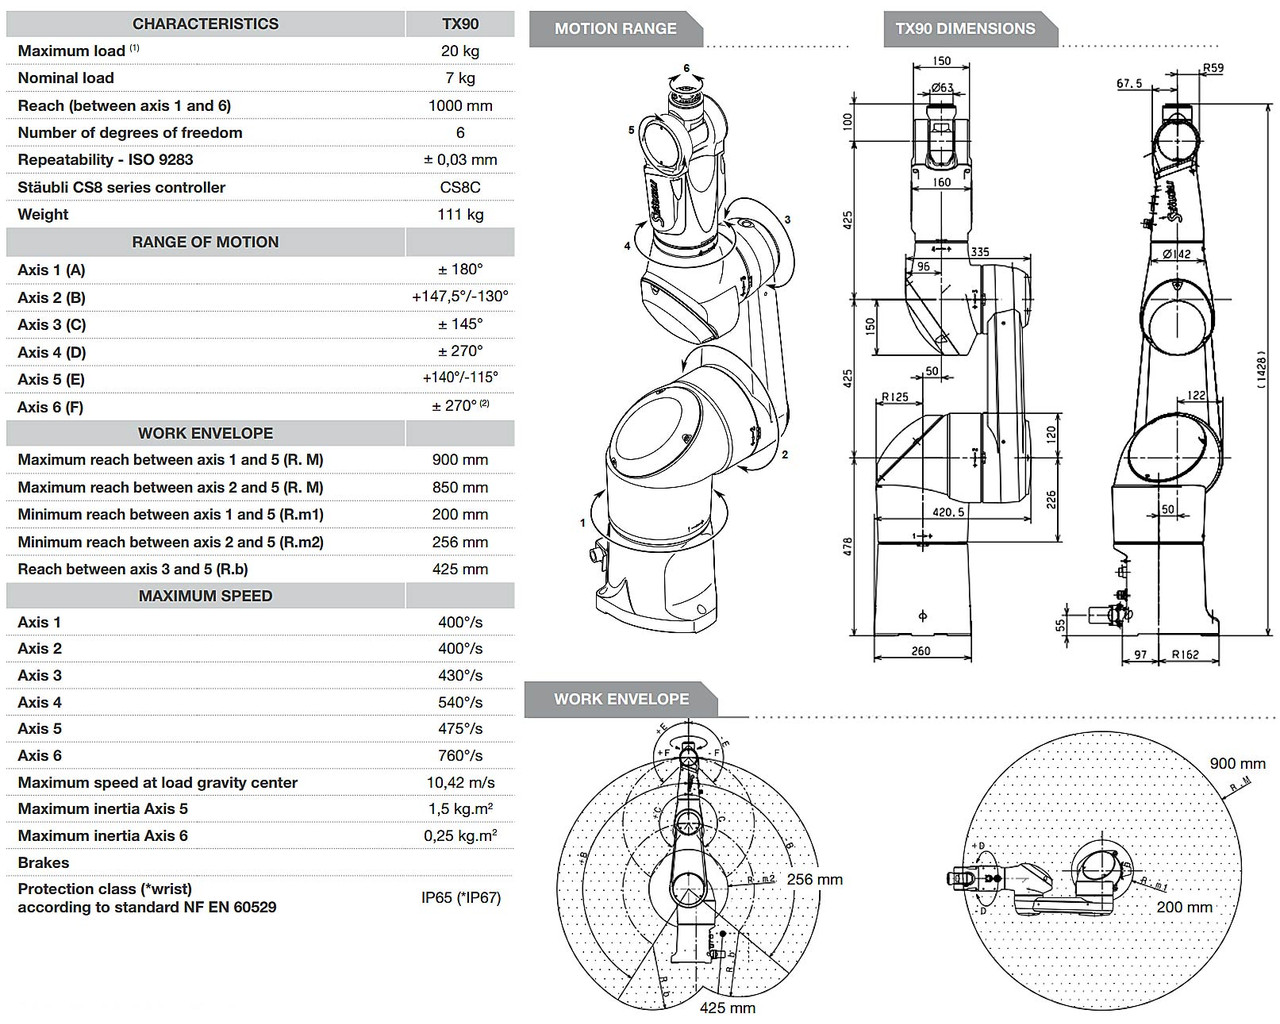
\includegraphics[width=0.92\linewidth]{dados_fonte/dados_staubli.png}
    \caption{Características, dimensões e limites de movimento do TX90.
    Fonte: \citeonline{staubli2017}.}
    \label{fig:dados_tecnicos_tx90}
\end{figure}
